\documentclass[11pt]{article}
\usepackage[sort]{natbib}
\usepackage{bm,amsmath,bbm,amsfonts,nicefrac,latexsym,amsmath,amsfonts,amsbsy,amscd,amsxtra,amsgen,amsopn,bbm,amsthm,amssymb,graphicx, breqn, setspace, printlen, caption, subcaption, pbox, fixltx2e}
\usepackage{fancyhdr, color}
\usepackage{mathptmx}     
\bibliographystyle{abbrvnat}
%\usepackage[section]{placeins}
\usepackage[margin=1.0in]{geometry}

\title{Chapter 2: Observability and Information Content {\color{red}DRAFT}}
\author{Ewan Pinnington}

\newtheorem{theorem}{Theorem}[section]
\newtheorem*{defn}{Definition}


\begin{document}

\maketitle

\section{Introduction (to be included in literature review chapter)}

\subsection{Observability}

Observability is a mathematical concept from control theory. A system is said to be observable if it is possible to determine the state by measuring only the output. The following definition is taken from \citet{barnett1985introduction}, For the linear time varying system defined as,
\begin{align}
\dot{\textbf{x}} &= \textbf{A}(t)\textbf{x}(t) +\textbf{B}(t)\textbf{u}(t) \\
\textbf{y} &= \textbf{C}(t)\textbf{x}(t)
\end{align}
where $\textbf{A}$ is $n \times n$, $\textbf{B}$ is $n \times m$ and $\textbf{C}$ is $r \times n$ is \textit{completely observable} if for any $t_0$ and any initial state $\textbf{x}(t_0) = \textbf{x}_0$ there exists a finite time $t_i > t_0$ such that knowledge of $\textbf{u}(t)$ and $\textbf{y}(t)$ for $t_0 \leq t \leq t_i$ suffices to uniquely determine $\textbf{x}_0$. There is no loss of generality in assuming $\textbf{u}(t)$ is identically zero throughout the whole interval, this is the case for data assimilation.

\begin{theorem} \label{thm:observable}
When $\textbf{A}$, $\textbf{B}$ and $\textbf{C}$ are time-invariant the system is completely observable if and only if the $nr \times n$ observability matrix
\begin{equation}
\mathbf{V}=
\begin{pmatrix}
\mathbf{C} \\
\mathbf{C}\mathbf{A}\\
\mathbf{C}\mathbf{A}^{2}\\
\vdots \\
\mathbf{C}\mathbf{A}^{n-1}
\end{pmatrix}
\end{equation}
has rank $n$.
\end{theorem}

This result can be applied to the data assimilation problem \citep{johnson2005singular}, where for 4D-Var the observability matrix corresponds to
\begin{equation}
\hat{\mathbf{H}}=
\begin{pmatrix}
\mathbf{H}_0 \\
\mathbf{H}_1\mathbf{M}_0\\
\vdots \\
\mathbf{H}_N\mathbf{M}_{N,0}
\end{pmatrix} \label{eqn: hmat}
\end{equation}
as defined in section {\color{red} REF}. So that if the rank of $\hat{\textbf{H}}$ is equal to $n$, the size of $\textbf{x}_0$, the system is observable. Theorem \ref{thm:observable} is for linear systems and has been applied to the linearised data assimilation problem. For a set of observations $\hat{\textbf{y}}$ this still gives us a good indication to the observability of the system, although it is not a measure of non-linear observability. It is important to note that the system being observable in this case means that we can construct a unique solution from the observational part of the cost function and does not account for parameter miss-specification and observation error. In \citet{Cohn1988} it is shown that having an observable system is necessary and sufficient for asymptotic stability of the data assimilation process. In practice we include a background term in the cost function for 4D-Var data assimilation which regularises the problem and means that we always have a unique solution.

\section{Information Content Measures}%%%%%%%%%%%%%%%%%%%%%%

Information content measures are already being used to quantify the different levels of information provided by observations in the development of satellite instruments \citep{stewart2008correlated, engelen2004information} and in operational data assimilation schemes \citep{fisher2003estimation, singh2013practical}. In these fields, two of the more widely used measures are Shannon Information Content (also known as entropy reduction) and the degrees of freedom for signal. We will apply both methods for observations assimilated with DALEC. 

\subsection{Shannon Information Content}%%%%%%%%%%%%%%%%%%%%%%

In DA, Shannon Information Content ($SIC$) is a measure of the reduction in entropy given a set of observations. Entropy physically corresponds to the volume in state space taken up by the probability density function ($pdf$) describing the knowledge of the state. When a measurement is made, the volume of this $pdf$ decreases. The $SIC$ of the measurement is a measure of the factor by which the $pdf$ decreases \citep{rodgers2000inverse}. If $P_b(x)$ is our knowledge of the state before an observation and $P_o(x|y)$ is our knowledge after an observation then we have entropies,
\[
S[P_b(x)] = - \int P_b(x)\text{log}_2[P_b(x)]dx
 \hspace{5mm} \text{and} \hspace{5mm} 
S[P_o(x|y)] = - \int P_o(x|y)\text{log}_2[P_o(x|y)]dx.
\]
The entropy reduction, or $SIC$, due to the observation is then,
\begin{equation} \label{shaic}
SIC =  S[P_b(x)]-S[P_o(x|y)].
\end{equation}
If we assume all $pdfs$ are Gaussian and use the natural logarithm as opposed to $\text{log}_2$ (for algebraic convenience) \cite{rodgers2000inverse}, the entropy of a multivariate Gaussian distruibution for a vector $\textbf{x}$ with $n$ elements (before and after observations) can be derived as,
\begin{equation} \label{SB}
 S[P_b(\textbf{x})] = n\text{ln}(2\pi e)^{\frac{1}{2}}+\frac{1}{2}\text{ln}\begin{vmatrix}\bf{B}\end{vmatrix}
\end{equation}
and
\begin{equation} \label{SA}
 S[P_o(\textbf{x}|\textbf{y})] = n\text{ln}(2\pi e)^{\frac{1}{2}}+\frac{1}{2}\text{ln}\begin{vmatrix}\bf{A}\end{vmatrix}
\end{equation}
where $\bf{B}$ is the background error covariance matrix and $\bf{A}$ is the analysis error covariance matrix. Combining equations \ref{shaic}, \ref{SB} and \ref{SA} we can write the $SIC$ as,
\begin{equation}
SIC=\frac{1}{2}\text{ln}\frac{\begin{vmatrix} \bf{B} \end{vmatrix}}{\begin{vmatrix} \bf{A} \end{vmatrix}}.
\end{equation}•
From equation \ref{Amat} we can see the $SIC$ can also be written as,
\begin{equation}
SIC= \frac{1}{2}\text{ln}\begin{vmatrix} \mathbf{B} \end{vmatrix}\begin{vmatrix} \mathbf{J}'' \end{vmatrix}. \label{sic}
\end{equation}•

\subsection{Degrees of Freedom for Signal} \label{DFSintro}%%%%%%%%%%%%%%%%%%%%%%

The degrees of freedom for signal ($DFS$) indicates the number of elements of the state that have been measured by the observations. If we consider a state vector $\textbf{x}$ with $n$ elements (or $n$ degrees of freedom) then the maximum value the $DFS$ could obtain would be $n$, in this case all elements of the state would have been measured. Conversely if $DFS = 0$ then no elements of the state would have been measured by our observations \citep{Fowler2013}.

We have symmetric positive definite background and analysis error covariance matrices $\bf{B}$ and $\bf{A}$. The eigenvalues of each matrix gives a representation for the uncertainty in the direction of the associated eigenvector, thus, by comparing the eigenvalues of both matrices we can determine the reduction in uncertainty given a set of observations \citep{stewart2008correlated}.

In order to do this we take $\mathbf{B}^{\frac{-1}{2}}$ such that $\mathbf{B}^{-1} = \mathbf{B}^{\frac{-1}{2}}\mathbf{B}^{\frac{-1}{2}}$. We now take $\bf{Q}$ to be the orthogonal matrix composed of the eigenvectors of $\mathbf{B}^{\frac{-1}{2}}\mathbf{A}\mathbf{B}^{\frac{-1}{2}}$ we have,
\begin{equation}
\mathbf{Q}^{T}\bigg(\mathbf{B}^{\frac{-1}{2}}\mathbf{A}\mathbf{B}^{\frac{-1}{2}}\bigg)\mathbf{Q} = \bf{\Lambda},
\end{equation}• 
\begin{equation}
\mathbf{Q}^{T}\bigg(\mathbf{B}^{\frac{-1}{2}}\mathbf{B}\mathbf{B}^{\frac{-1}{2}}\bigg)\mathbf{Q} = \mathbf{I}_{n\times n}
\end{equation}•
where $\bf{\Lambda}$ is a diagonal matrix. Each diagonal element of our transformed $\bf{B}$ is equal to one and corresponds to one degree of freedom. The diagonal elements of $\mathbf{\Lambda}$ correspond to the matrix's eigenvalues and can be interpreted as the relative reduction in variance for each of the $n$ degrees of freedom \cite{singh2013practical}. We can then define the $DFS$ as,
\begin{equation}
\begin{split}
DFS & = \text{trace}(\mathbf{I}_{n\times n} - \mathbf{\Lambda}) \\
       & = n - \text{trace}(\mathbf{\Lambda}) \\
       & = n - \text{trace}(\mathbf{B}^{\frac{-1}{2}}\mathbf{A}\mathbf{B}^{\frac{-1}{2}}) \\
       & = n - \text{trace}(\mathbf{B}^{-1}\mathbf{A}).
\end{split}
\end{equation}

\subsection{Look at Christine Johnsons paper and CVT Hhat for obs impact?}

\subsection{Cardinalli influence matrix to show spreading of information from correlations}


\section{Results}

\subsection{DALEC1 observability} \label{sec:D1observability}

DALEC1 is the original version of the DALEC2 model introduced in section {\color{red} REF}. At the start of the PhD project work was undertaken with DALEC1 before the DALEC2 model was released. The version of DALEC1 used was an evergreen only model, further details of the model can be found in section {\color{red} REF} and \citet{williams2005improved}. 

We initially consider observability of the DALEC1 state estimation system. DALEC1 is a smaller model and allows us to understand the concept of observability before moving onto work with the more complicated DALEC2 joint state and parameter estimation system. DALEC1 was implemented in a 4D-Var data assimilation scheme for state estimation, with the tangent linear model being computed analytically by hand. Using this analytic implementation of the tangent linear model we can compute the observability of the model for differing sets of observations. We have the tangent linear model,
\begin{dmath}
\mathbf{M}_{i} = \frac{\partial \textbf{m}_{i-1\rightarrow i}(\textbf{x}_{i})}{\partial \textbf{x}_{i}} = 
\begin{pmatrix}  
(1-\theta_{fol})+f_{fol}(1-f_{auto})\zeta^i & 0 & 0 & 0 & 0 \\
f_{roo}(1-f_{fol})(1-f_{auto})\zeta^i & (1-\theta_{roo}) & 0 & 0 & 0 \\
(1-f_{roo})(1-f_{fol})(1-f_{auto})\zeta^i & 0 & (1-\theta_{woo}) & 0 & 0 \\
\theta_{fol} & \theta_{roo} & 0 & (1-(\theta_{min}+\theta_{lit})\chi^{i-1}) & 0 \\
0 & 0 & \theta_{lit} & \theta_{min}\chi^{i-1} & (1-\theta_{som}\chi^{i-1}) \\
\end{pmatrix}, \label{eqn:linmod}
\end{dmath}
where \(\textbf{x}_{i}=(C_{fol}^{i}, C_{roo}^{i}, C_{woo}^{i}, C_{lit}^{i}, C_{som}^{i})^{T}\), $\zeta^i = \frac{\partial GPP^{i}(C_{fol}^{i-1}, \Psi)}{\partial C_{fol}^{i-1}}$ and $\chi^{i-1}=e^{\Theta T^{i-1}}$ with the parameters and symbols having the same meaning as in section {\color{red} REF}. 

We can use the linearised model with the linearised observation operator $\textbf{H}_{i}$ to form the matrix in equation~\ref{eqn: hmat} and compute the observability. We will need at least 5 observations of any type for the system to be observable as the state $\textbf{x}_0$ is of size 5 in the DALEC1 state estimation case. We first consider the observability for 5 observations of LAI. For DALEC1 LAI takes the form
\begin{equation}
LAI^{i} = \frac{C_{fol}^{i}}{c_{lma}}.
\end{equation}
We then have the linearised observation operator
\begin{equation}
\textbf{H}_{i} = \frac{\partial LAI^{i}}{\partial \textbf{x}_{i}} =
\begin{pmatrix}
\frac{1}{c_{lma}} & 0 & 0 & 0 & 0
\end{pmatrix}.
\end{equation}
Using the linearised observation operator and the linear model from equation~\ref{eqn:linmod} we can compute $\hat{\textbf{H}}$ for 5 observations of LAI with
\begin{dmath}
\hat{\mathbf{H}} =
\begin{pmatrix}
\mathbf{H}_0 \\
\mathbf{H}_1\mathbf{M}_0 \\
\vdots \\
\mathbf{H}_{4}\mathbf{M}_{3,0}

\end{pmatrix}
=
\begin{pmatrix}
\frac{1}{c_{lma}} & 0 & 0 & 0 & 0 \\
\frac{1}{c_{lma}}((1-\theta_{fol})+f_{fol}(1-f_{auto})\zeta^0) & 0 & 0 & 0 & 0 \\
\frac{1}{c_{lma}}\prod_{i=0}^{1}((1-\theta_{fol})+f_{fol}(1-f_{auto})\zeta^i) & 0 & 0 & 0 & 0 \\
\frac{1}{c_{lma}}\prod_{i=0}^{2}((1-\theta_{fol})+f_{fol}(1-f_{auto})\zeta^i) & 0 & 0 & 0 & 0 \\
\frac{1}{c_{lma}}\prod_{i=0}^{3}((1-\theta_{fol})+f_{fol}(1-f_{auto})\zeta^i) & 0 & 0 & 0 & 0
\end{pmatrix},
\end{dmath}
so that no matter how many observations of LAI we add our system will not be observable as the rows of $\hat{\textbf{H}}$ are all linearly dependant, so that $\hat{\textbf{H}}$ in this case has rank 1. We can repeat this for different observations to see for which observation types our system is observable. 

\begin{figure}[ht]
    \centering
    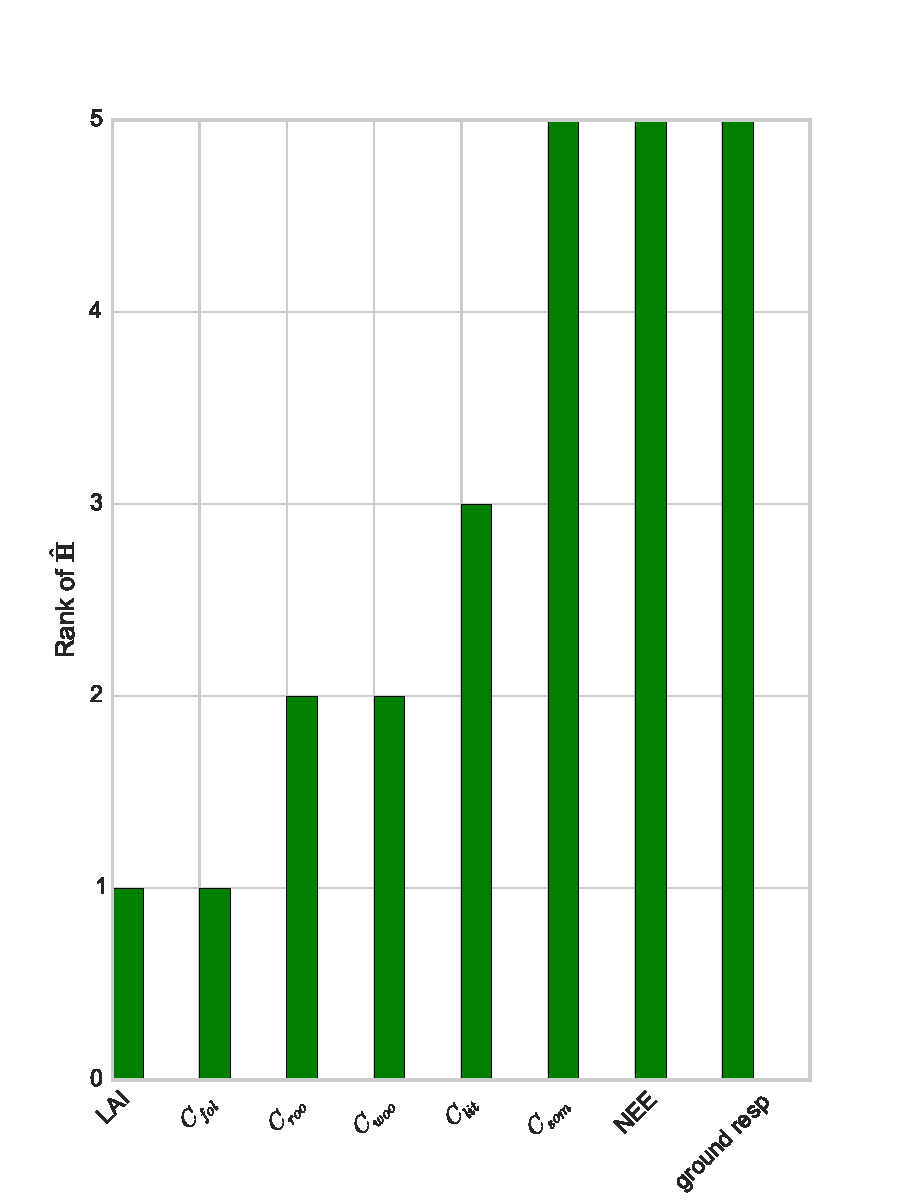
\includegraphics[width=0.5\textwidth]{dalec1_obsrank.pdf}
    \caption{Rank of the observability matrix $\hat{\textbf{H}}$ for 5 observations of different types. The ranks shown here are computed analytically using SymPy \citep{Joyner:2012:OSC:2110170.2110185}.}
    \label{fig:D1_observability}
\end{figure}

From figure~\ref{fig:D1_observability} we can see that our system is observable for 5 observations of the soil and organic matter carbon pool $C_{som}$. In figure~\ref{fig:D1_observability} we have shown results for the rank of  $\hat{\textbf{H}}$ when we have 5 observations in each case, this has also been tested with increasing numbers of observations being added to the system with the results from figure~\ref{fig:D1_observability} remaining unchanged. 

The system being observable for observations of $C_{som}$ physically makes sense as all the carbon in the system that is not respired to the atmosphere eventually ends up in $C_{som}$, so that by taking observations of this pool we observe all the others. In a similar way $\hat{\textbf{H}}$ is also full rank for observations of NEE and ground respiration. We can see from the form of these observations in DALEC1 that they both contain indirect observations of $C_{som}$ with NEE taking the form
\begin{equation}
NEE^{i}=-(1-f_{auto})GPP^{i}(C_{fol}^{i-1}, \Psi) + \theta_{lit}C_{lit} e^{\Theta T^{i}} + \theta_{som}C_{som} e^{\Theta T^{i}} \label{eqn: D1_nee}
\end{equation}
with a corresponding linearised observation operator
\begin{equation}
\textbf{H}_{i} = \frac{\partial NEE^{i}}{\partial \textbf{x}_{i}} =
\begin{pmatrix}
-(1-f_{auto})\zeta^i & 0 & 0 & \theta_{lit} e^{\Theta T^{i}} & \theta_{som} e^{\Theta T^{i}}
\end{pmatrix},
\end{equation}
and for ground respiration
\begin{equation}
G_{resp}^{i}=\frac{1}{3}f_{auto}GPP^{i}(C_{fol}^{i-1}, \Psi) + \theta_{lit}C_{lit} e^{\Theta T^{i}} + \theta_{som}C_{som} e^{\Theta T^{i}} \label{neeeqn}
\end{equation}
(here we have assumed the fraction of total autotrophic respiration from below ground to be $\frac{1}{3}$) with a corresponding linearised observation operator
\begin{equation}
\textbf{H}_{i} = \frac{\partial G_{resp}^{i}}{\partial \textbf{x}_{i}} =
\begin{pmatrix}
\frac{1}{3}f_{auto}\zeta^i & 0 & 0 & \theta_{lit} e^{\Theta T^{i}} & \theta_{som} e^{\Theta T^{i}}
\end{pmatrix}.
\end{equation}
At flux tower sites NEE is the most observed quantity, these results give us confidence that we can construct a unique solution when working with flux tower data. We will further explore the concept of observability for the joint parameter and state estimation case with DALEC2 in section~\ref{sec: D2_observability}. 

For the state and parameter estimation case we will not be able to compute the observability of the system analytically, it is therefore important to check that the numerical calculation of the rank of $\hat{\textbf{H}}$ for DALEC1 is equal to the rank when calculated analytically. This will give us confidence that our implementation of the numeric rank is correct for DALEC2 as the implementation is the same in both cases. In table~\ref{table: a_n_h_D1} we show that for both numeric and analytic implementations we have the same results for the rank of $\hat{\textbf{H}}$.

\begin{table}[ht] 
\begin{center}
	\begin{tabular}{| l | l | l | l}
	\hline
	Observation & Rank of $\hat{\textbf{H}}$ (numeric) & Rank of $\hat{\textbf{H}}$ (analytic) \\ \hline
	LAI & 1 & 1 \\ \hline
	$C_{fol}$ & 1 & 1  \\ \hline
	$C_{roo}$ & 2 & 2 \\ \hline
	$C_{woo}$ & 2 & 2 \\ \hline
	$C_{lit}$ & 3 & 3 \\ \hline
	$C_{som}$ & 5 & 5 \\ \hline
	NEE & 5 & 5 \\ \hline
	$G_{resp}$ & 5 & 5 \\  
	\hline
	\end{tabular}
	\caption{Rank of $\hat{\textbf{H}}$ for 5 observations of different types for both numeric and analytic implementations with DALEC1.}
	\label{table: a_n_h_D1}
\end{center} 
\end{table}

% \subsection{DALEC1 information content}

\subsection{DALEC2 observability} \label{sec: D2_observability}

For DALEC2 we perform joint parameter and state estimation and have an augmented state of size $n = 23$. The augmented state is made up of the 6 carbon pool state members and 17 model parameters as described in section~{\color{red} REF}. As we are also estimating the parameters of DALEC2 the concept of observability for our system is closely linked to the concept of identifiability \citep{navon1998practical}. A system is identifiable if given observations of the state variables and knowledge of the model dynamics it is possible to obtain a unique deterministic set of model parameter values \citep{ljung1998system}. If a model parameter is not observable it will not be identifiable \citep{Jacquez1985}. It is therefore useful to compute the observability of the DALEC2 joint parameter and state estimation system.

We compute observability in the same way as in section~\ref{sec:D1observability} by finding the rank of $\hat{\textbf{H}}$ for a given set of observations. As discussed in section~\ref{sec:D1observability} we cannot compute the observability analytically for the DALEC2 joint parameter and state estimation scheme. We have tested our numeric implementation for the state estimation case with DALEC1 and find the same results for the rank of $\hat{\textbf{H}}$ as for the analytic case. We calculate the rank of the $\hat{\textbf{H}}$ matrix using a singular value decomposition (SVD) which can have issues if the condition number of $\hat{\textbf{H}}$ is large \citep{Paige1981}. This is a problem we encounter in the DALEC2 case when trying to calculate the rank of $\hat{\textbf{H}}$ directly.  

\begin{figure}[ht]
    \centering
    \begin{subfigure}[b]{0.49\textwidth}
        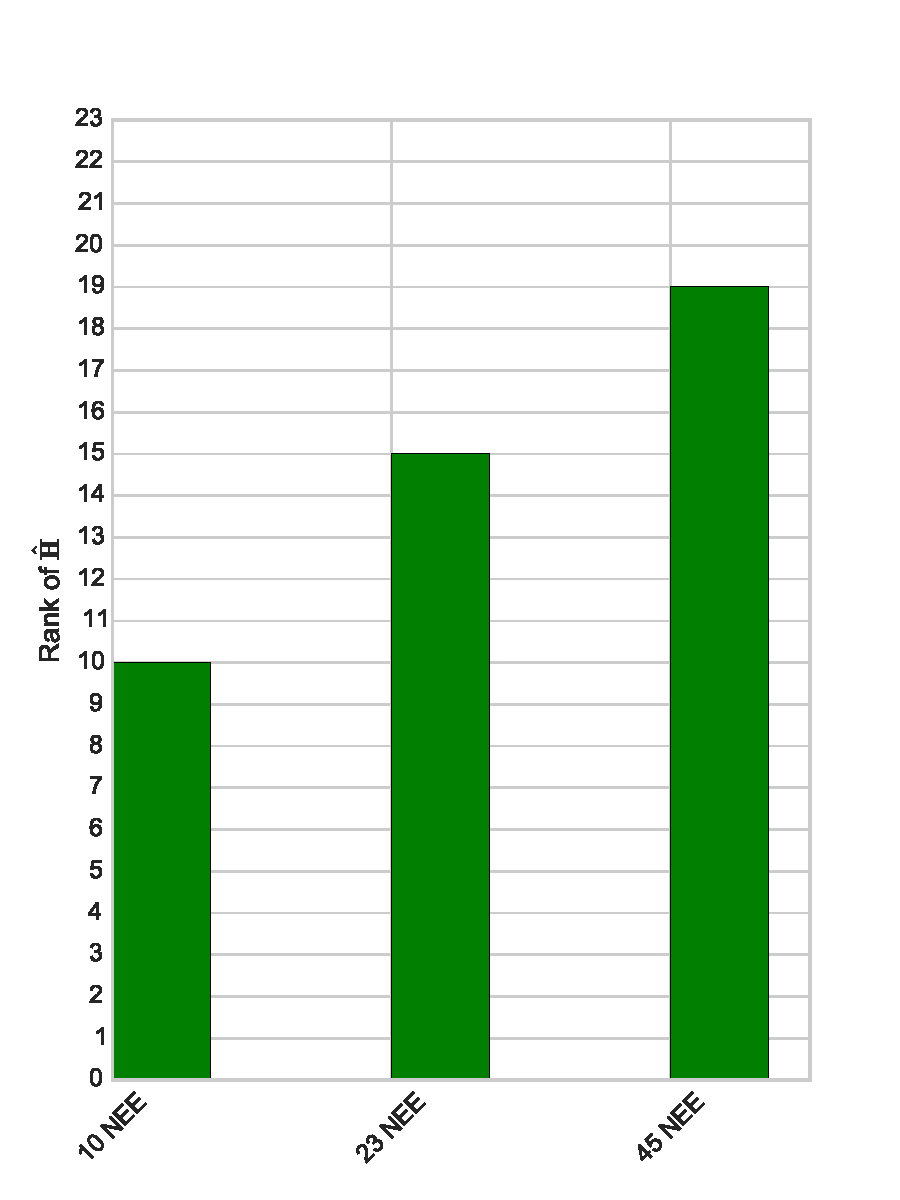
\includegraphics[width=\textwidth]{dalec2_obsrank.pdf}
        \caption{Rank of $\hat{\textbf{H}}$}
        \label{fig:D2_observabilityrank}
    \end{subfigure}
    \begin{subfigure}[b]{0.49\textwidth}
        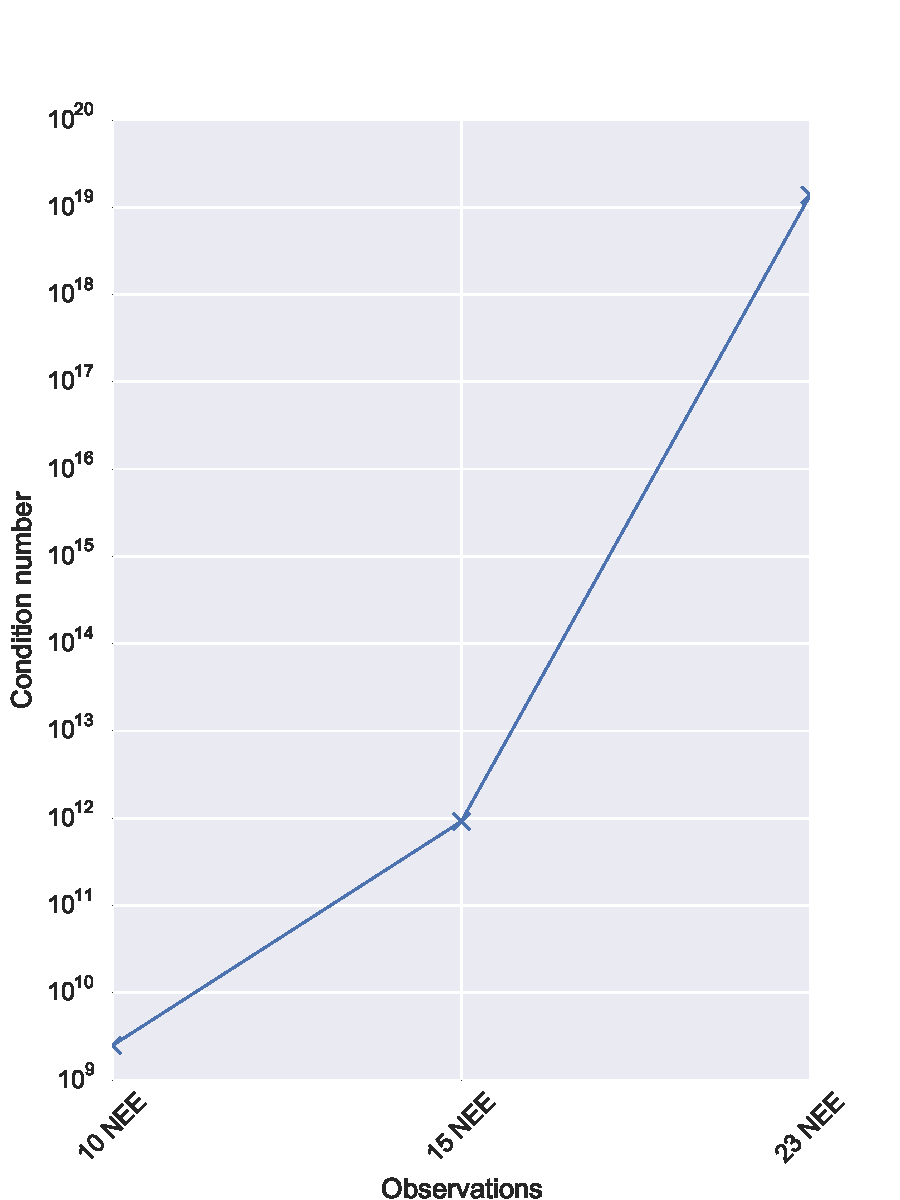
\includegraphics[width=\textwidth]{dalec2_obsrankcond.pdf}
        \caption{Condition number of $\hat{\textbf{H}}$}
        \label{fig:D2_observabilitycond}
    \end{subfigure}
    \caption{Observability of DALEC2 for $\hat{\textbf{H}}$ with an increasing number of NEE observations displayed alongside the condition number for the $\hat{\textbf{H}}$ matrices.}
    \label{fig:D2_observability}
\end{figure}

In figure~\ref{fig:D2_observabilityrank} we see that for 23 observations of NEE our system is unobservable as we have a rank deficient $\hat{\textbf{H}}$. However, we cannot trust the rank calculation of $\hat{\textbf{H}}$ in this case. Figure~\ref{fig:D2_observabilitycond} shows that for 23 observations of NEE $\hat{\textbf{H}}$ has a condition number in the order of $10^{19}$. The condition number of a matrix corresponds to the ratio of the largest to the smallest singular values. A condition number of this size means that we have very small singular values. In the calculation of the rank of a matrix using an SVD we define the rank to be the number of singular values greater than the threshold \texttt{ tol = max(S) * max(n, m) * eps } \citep{press2007numerical}, where \texttt{S} is the vector of singular values, \texttt{n} and \texttt{m} are the rows and columns of the matrix whose rank we wish to calculate and \texttt{eps} is the epsilon value for the datatype of \texttt{S} (In this case a double-precision float with \texttt{eps = 2.22e-16}). For 23 observations of NEE $\hat{\textbf{H}}$ is classed as being rank deficient as \texttt{tol = 1.02e-10} and the three smallest singular values of $\hat{\textbf{H}}$ are \texttt{[1.39e-11, 7.84e-15, 1.46e-15]} but here we are working past the accuracy of the computer and so cannot have confidence that $\hat{\textbf{H}}$ is rank deficient in this case.

\begin{figure}[ht]
    \centering
    \begin{subfigure}[b]{0.49\textwidth}
        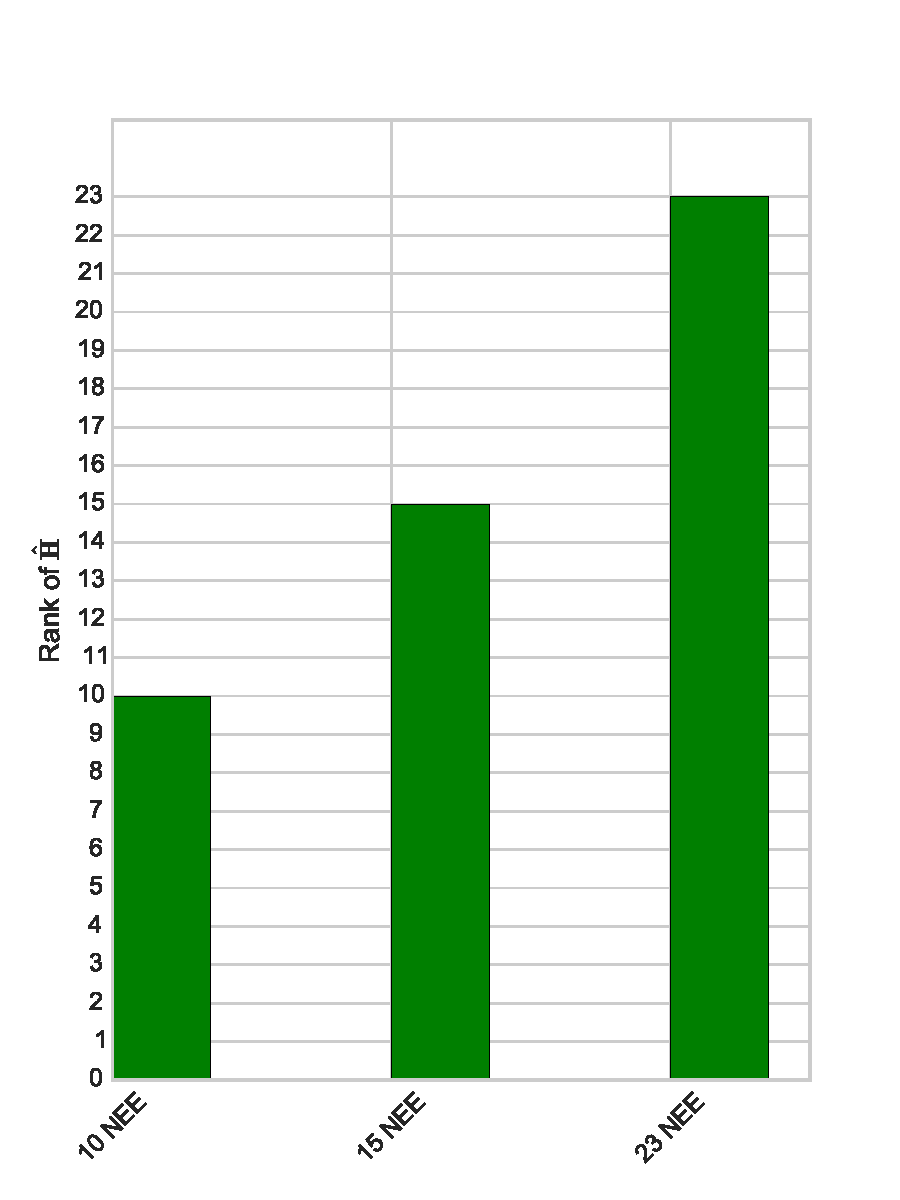
\includegraphics[width=\textwidth]{dalec2_obsrankcvt.pdf}
        \caption{Rank of $\hat{\textbf{R}}^{-1/2}\hat{\textbf{H}}\textbf{D}^{1/2}$}
        \label{fig:D2_observailityrankcvt}
    \end{subfigure}
    \begin{subfigure}[b]{0.49\textwidth}
        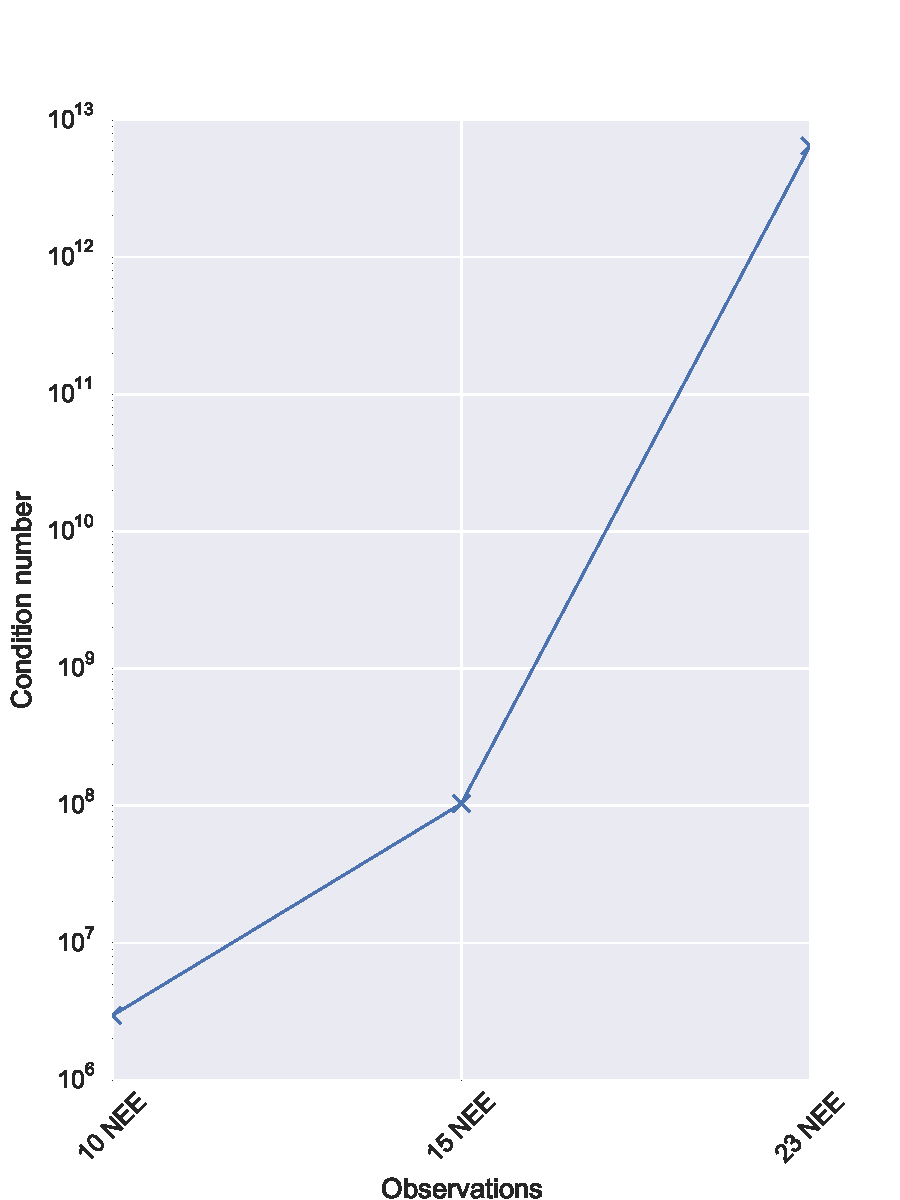
\includegraphics[width=\textwidth]{dalec2_obsrankcvtcond.pdf}
        \caption{Condition number of $\hat{\textbf{R}}^{-1/2}\hat{\textbf{H}}\textbf{D}^{1/2}$}
        \label{fig:D2_observabilitycondcvt}
    \end{subfigure}
    \caption{Observability of the CVT DALEC2 for $\hat{\textbf{R}}^{-1/2}\hat{\textbf{H}}\textbf{D}^{1/2}$ with an increasing number of NEE observations displayed alongside the condition number for the $\hat{\textbf{R}}^{-1/2}\hat{\textbf{H}}\textbf{D}^{1/2}$ matrices.}
    \label{fig:D2_cvtobservability}
\end{figure}

In order to address the problem of ill-conditioning of the $\hat{\textbf{H}}$ matrix we can instead calculate the rank of the control variable transform observability matrix, $\hat{\textbf{R}}^{-1/2}\hat{\textbf{H}}\textbf{D}^{1/2}$, where the symbols have the same meaning as in section {\color{red} REF section where CVT is described, $\textbf{D} = diag\{\textbf{B}\}$}. From figure~\ref{fig:D2_observabilitycondcvt} we can see this matrix is much better conditioned than $\hat{\textbf{H}}$ and for 23 observations of NEE we now have an observable system. Although the condition numbers here are still large we can have more confidence in these results as we are working within the precision of the computer.

In the previous experiments we have considered increasing numbers of NEE observations taken on adjacent days. It is also useful to consider the observability of the system when we have a number of observations randomly distributed throughout a time window. This is more consistent with what we expect from the real data we have to work with.  

\begin{figure}[ht]
    \centering
    \begin{subfigure}[b]{0.49\textwidth}
        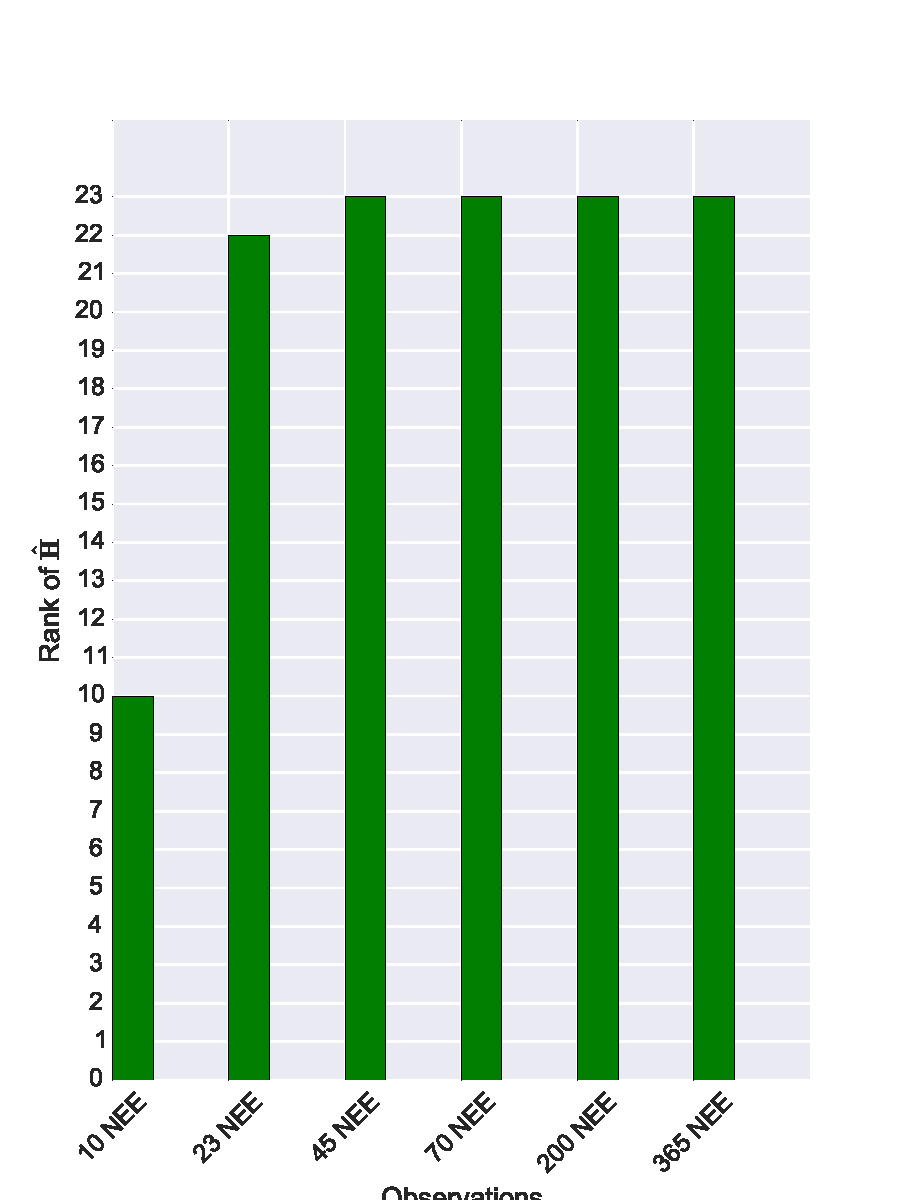
\includegraphics[width=\textwidth]{dalec2_obsrankwind.pdf}
        \caption{Rank of $\hat{\textbf{H}}$}
        \label{fig:D2_observailityrankwind}
    \end{subfigure}
    \begin{subfigure}[b]{0.49\textwidth}
        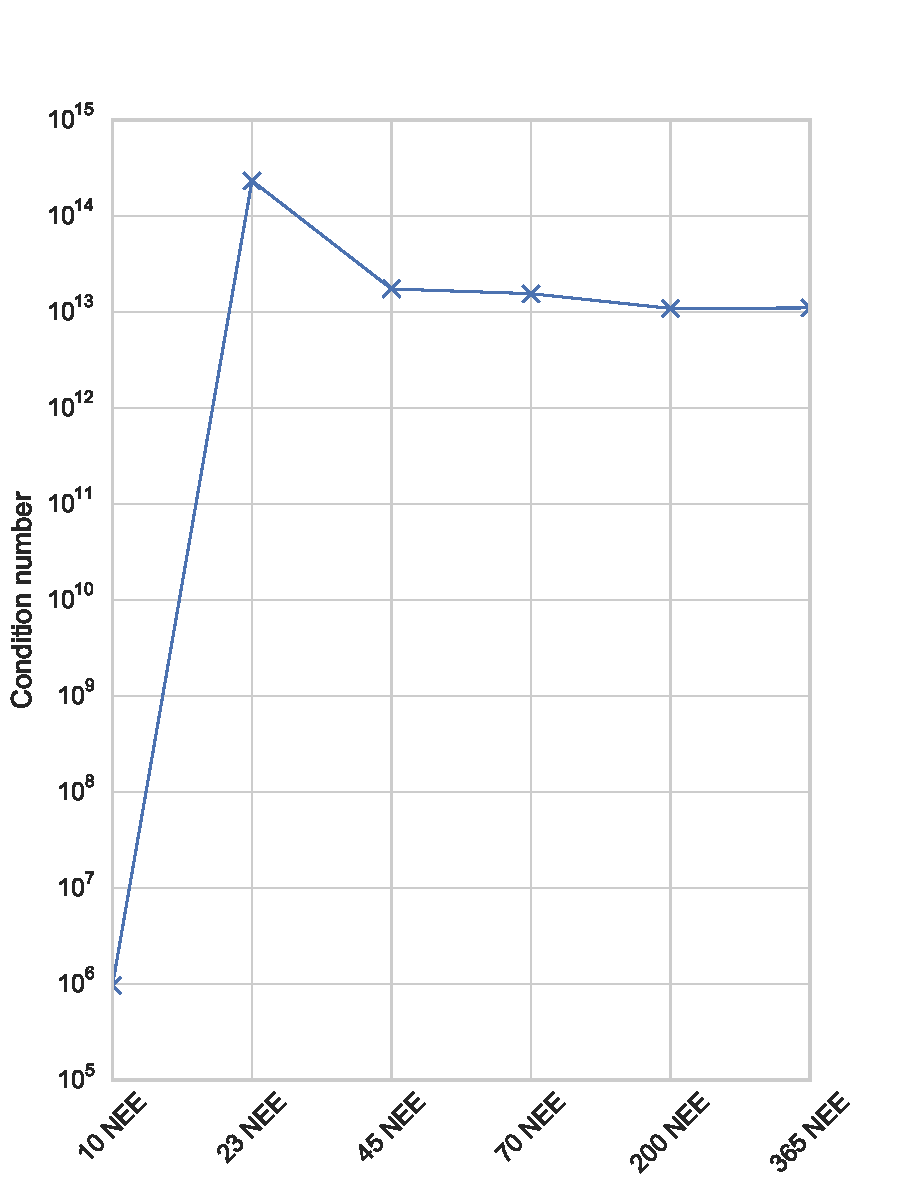
\includegraphics[width=\textwidth]{dalec2_obsrankcondwind.pdf}
        \caption{Condition number of $\hat{\textbf{H}}$}
        \label{fig:D2_observabilitycondwind}
    \end{subfigure}
    \caption{Observability of DALEC2 for a $\hat{\textbf{H}}$ with an increasing number of NEE observations randomly distributed through a 1 year assimilation window (left). Condition number for the $\hat{\textbf{H}}$ matrices (right).}
    \label{fig:D2_observabilitywind}
\end{figure}

In figure~\ref{fig:D2_observabilitywind} we see that having the observations randomly distributed throughout a 1 year assimilation window has improved the conditioning of $\hat{\textbf{H}}$ in comparison to figure~\ref{fig:D2_observability}. This is due to the observations being randomly distributed rather than adjacent. The rows of $\hat{\textbf{H}}$ are more distinct when being evolved to different times in the year by the tangent linear model rather than evolved to adjacent days only. However, we still have a rank deficient $\hat{\textbf{H}}$ for the 23 NEE observation case. From figure~\ref{fig:D2_observabilitycondwind} we see that this is the case where the condition number peaks. As we add more randomly distributed observations the condition number of $\hat{\textbf{H}}$ is reduced by an order of $10^{2}$ and we have a full rank $\hat{\textbf{H}}$. 

In figure~\ref{fig:D2_cvtobservabilitywind} we again see that using the CVT observability matrix has much improved the conditioning of the problem in comparison to figure~\ref{fig:D2_observabilitywind}. We now have that the DALEC2 system is observable when we have 23 observations of NEE randomly distributed throughout the 1 year assimilation window. We have more confidence that this is the case as the condition numbers for the CVT observability matrix are almost half the values of those for $\hat{\textbf{H}}$. We again see a similar pattern in figure~\ref{fig:D2_cvtobservabilitywind} for the condition numbers with a peak for 23 NEE observations and then a reduction of order $10^{2}$ when more observations are added. 

We have tested the observability of the system for observations of NEE when we have different driving data, linearising around different states and with different distributions of observations throughout our assimilation window and in every case we have an observable system given an adequate number of NEE observations (at least 23). We can therefore have confidence that for the available data, typically 60-80 observations of daily NEE for any years window, we can construct a unique solution with the observations alone.

\begin{figure}[ht]
    \centering
    \begin{subfigure}[b]{0.49\textwidth}
        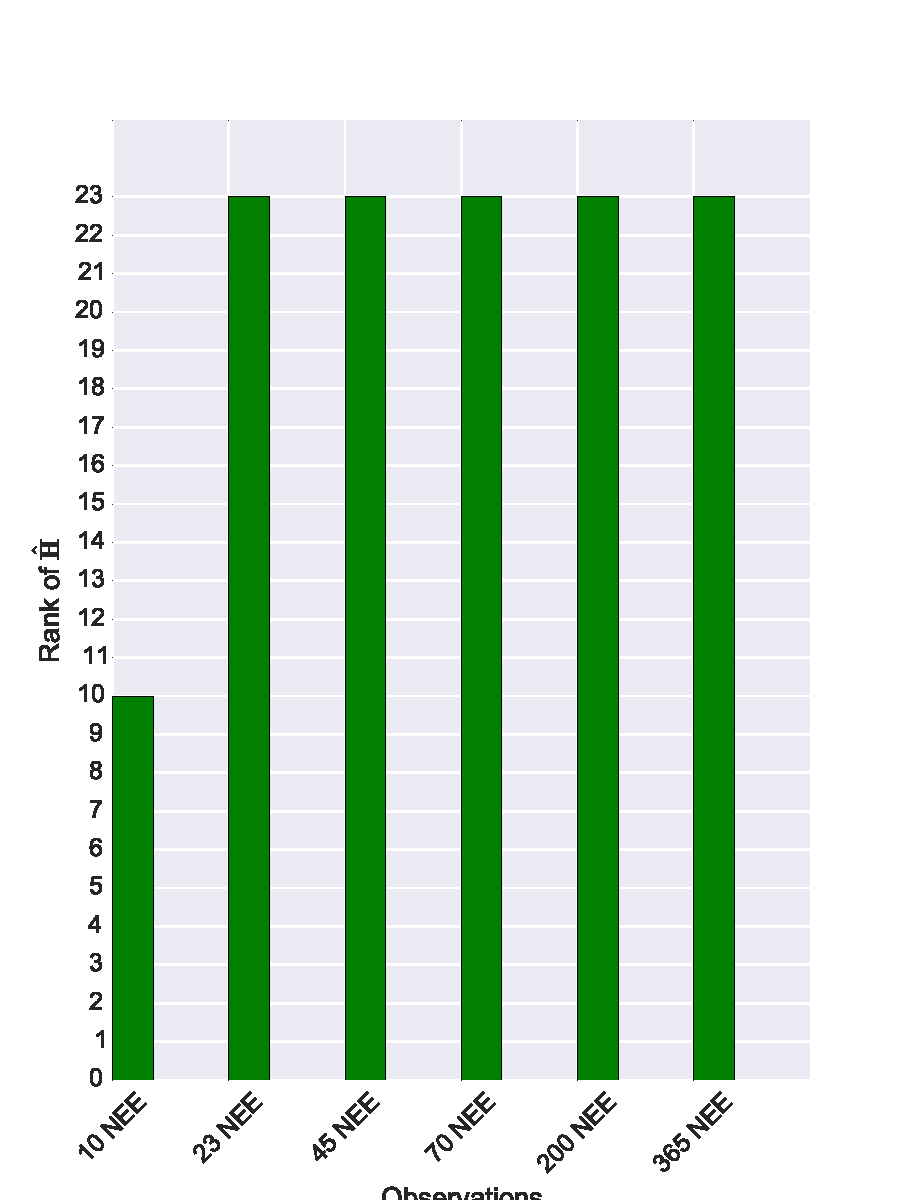
\includegraphics[width=\textwidth]{dalec2_obsrankcvtwind.pdf}
        \caption{Rank of $\hat{\textbf{R}}^{-1/2}\hat{\textbf{H}}\textbf{D}^{1/2}$}
        \label{fig:D2_observailityrankcvtwind}
    \end{subfigure}
    \begin{subfigure}[b]{0.49\textwidth}
        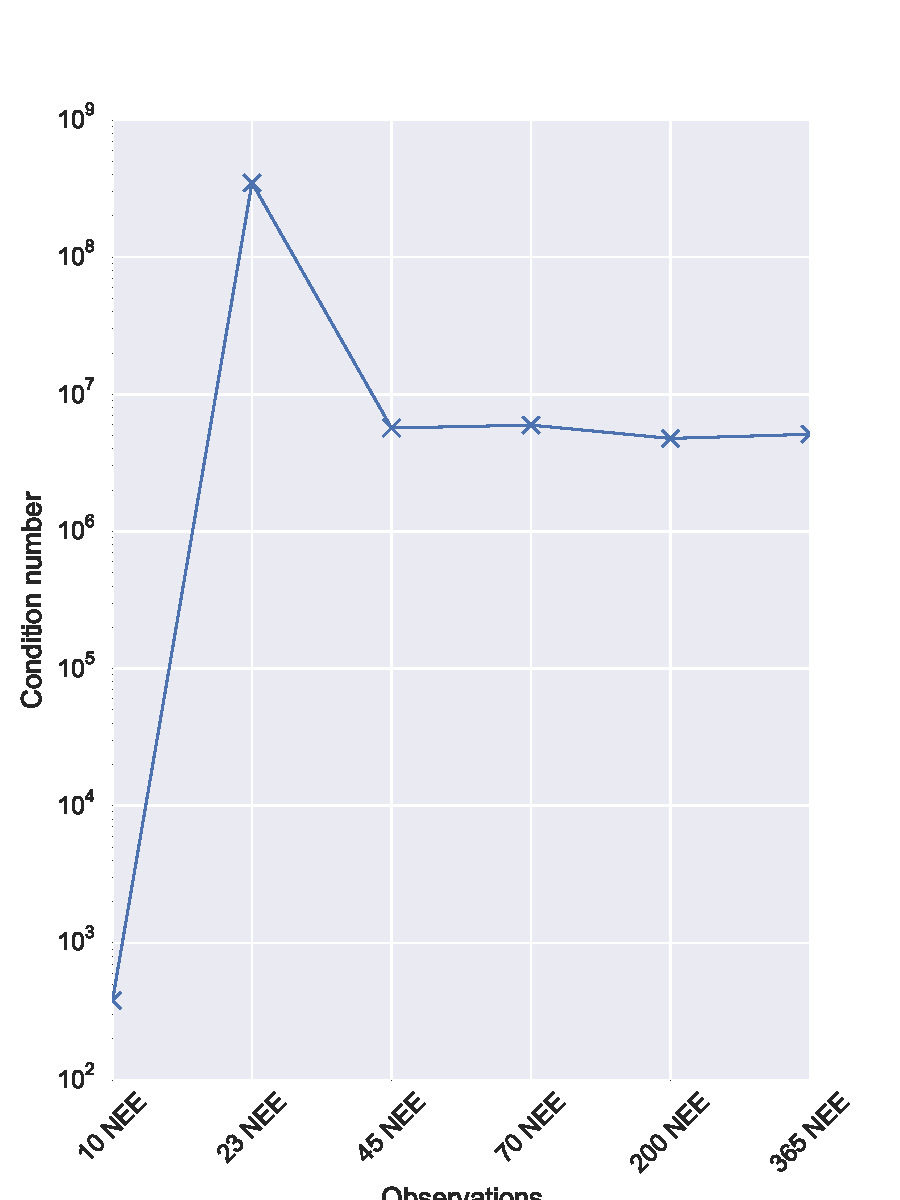
\includegraphics[width=\textwidth]{dalec2_obsrankcondcvtwind.pdf}
        \caption{Condition number of $\hat{\textbf{R}}^{-1/2}\hat{\textbf{H}}\textbf{D}^{1/2}$}
        \label{fig:D2_observabilitycondcvtwind}
    \end{subfigure}
    \caption{Observability of the CVT DALEC2 system for $\hat{\textbf{R}}^{-1/2}\hat{\textbf{H}}\textbf{D}^{1/2}$ with an increasing number of NEE observations randomly distributed through a 1 year assimilation window (left). Condition number for the $\hat{\textbf{R}}^{-1/2}\hat{\textbf{H}}\textbf{D}^{1/2}$ matrices (right).}
    \label{fig:D2_cvtobservabilitywind}
\end{figure}


\bibliography{../PhD}{}
\end{document}